\def\imanakacharacteristics{%
	\begin{itemize}
		\item 104 Patients
		\item Post op. immédiat de chx. card.
		\item Sédation profonde + paralysie
		%\item Mode VOIS + AI
		%\item Fr = 10\,/min, AI = 10\,hPa,
		%\item Vt = 6\,ml/kg, PEP = 4\,hPa
		%\item Seuil = 1 l/min
		\item 22 \% ont $\geq$  5 autodécl./min
	\end{itemize}
}

\def\imanakatable{%
	\begin{tabular}{lrl}
		%\hline
		Paramètre & \multicolumn{2}{l}{Valeur}\\
		\hline
		Mode & \multicolumn{2}{l}{VOI + AI}\\
		Seuil de décl. & 1 & l/m\\
		Fréquence & 10	& /min\\
		Aide inspiratoire	&	10 & mbar\\
		Volume courant & 6 & ml/kg\\
		PEP & 4 & mbar\\
		%\hline
	\end{tabular}
}

\begin{frame}{Imanaka et al. (2000)}
	\begin{columns}
		\column{0.45\textwidth}
		\imanakacharacteristics
		\vspace{\baselineskip}
		\hspace{20pt}\imanakatable
		\column{0.54\textwidth}
		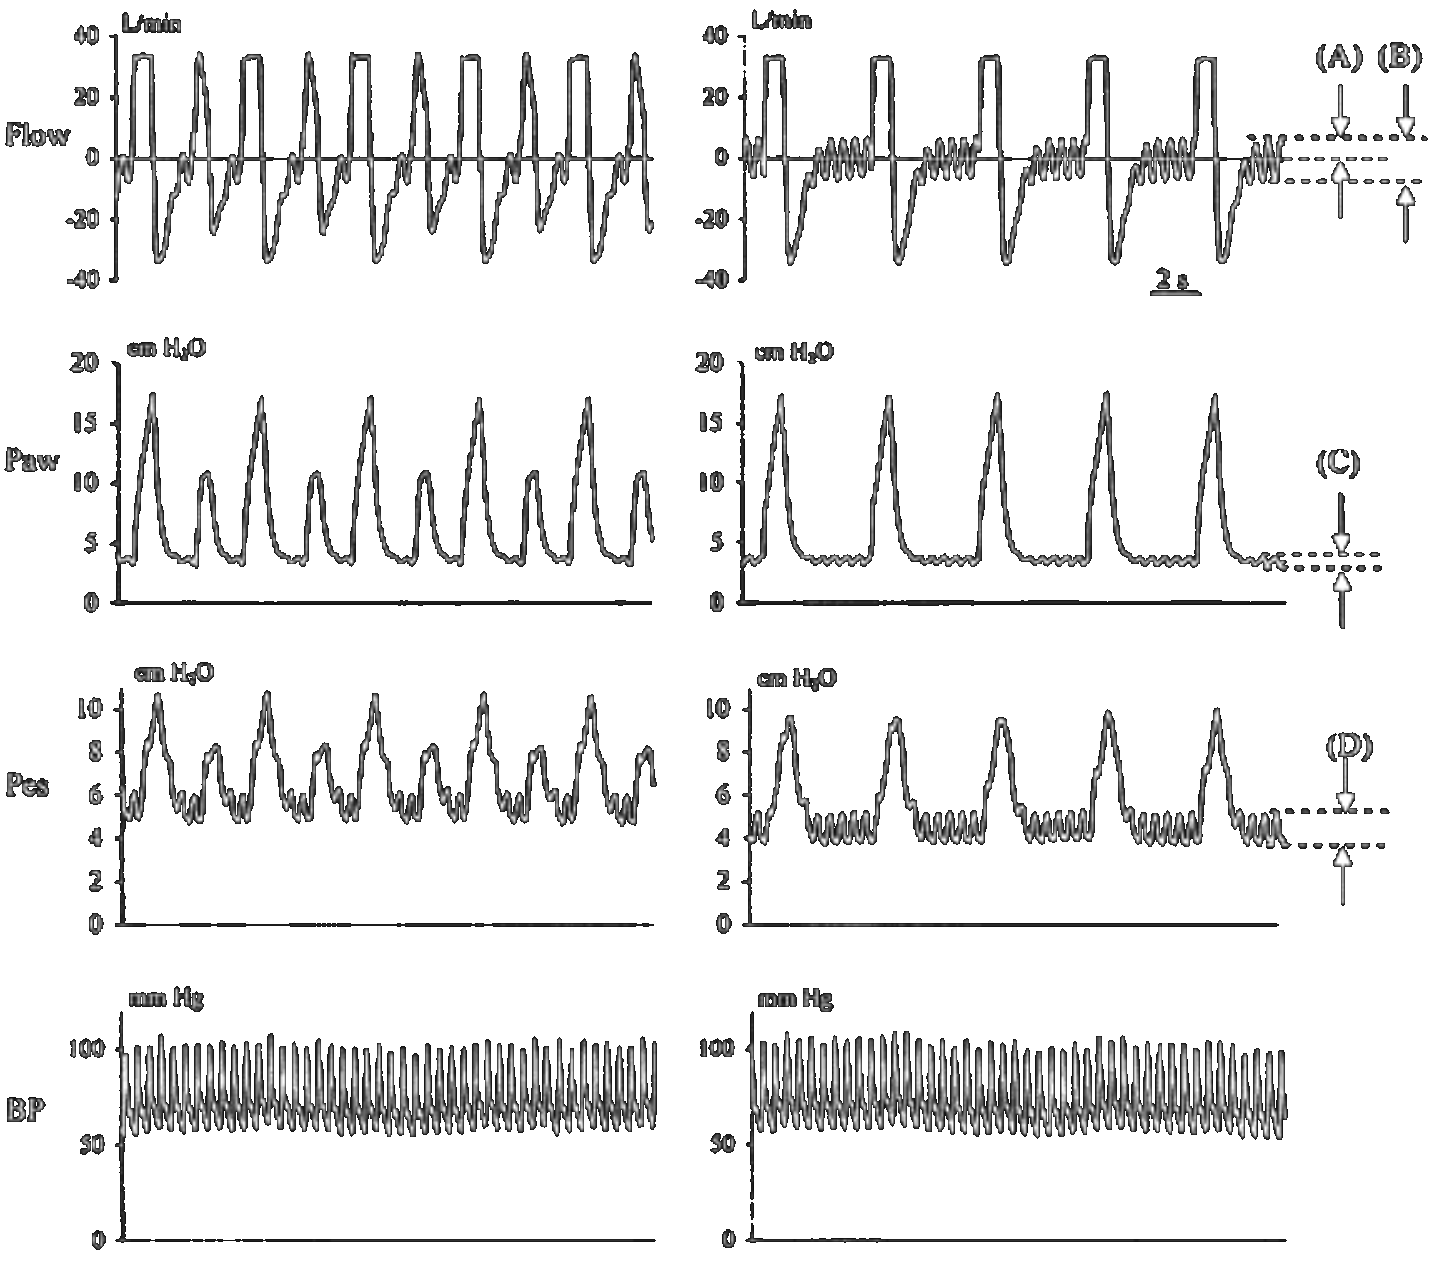
\includegraphics[width=\textwidth, clip, trim=0 90 107 0]{captures/Imanaka-transparent}
	\end{columns}
\end{frame}
